\documentclass{article}
\usepackage[spanish]{babel}
\usepackage[utf8]{inputenc}
\usepackage{amsfonts}
\usepackage{amsthm}
\usepackage{amsmath}
\usepackage{graphicx}
\usepackage{caption}
\usepackage{makeidx}
\usepackage{hyperref}
\setlength{\parindent}{0cm}
\bibliographystyle{IEEEtran}



\begin{document}

\title{Los tres grandes}
\author{Karlos Alejandro Alfonso Rodríguez C411\\Karel Camilo Manresa Leon C412}
\maketitle
\newpage

\section*{Resumen}
Este trabajo tiene como objetivo explorar la historia y la evolución de tres componentes electrónicos clave 
que han impulsado la revolución electrónica: el transistor, el circuito integrado y el microprocesador. 
Se abordará su desarrollo, características y aplicaciones, y explorará los avances tecnológicos 
recientes en electrónica que podrían tener un impacto significativo en la tecnología del futuro. 
La investigación cubre la historia del transistor desde su creación en la década de 1930, 
hasta la invención del primer transistor por William Shockley, John Bardeen y Walter Brattain en 1947, 
y sus posteriores avances. Además de la historia y el desarrollo del circuito integrado y el microprocesador, 
y su impacto en la electrónica moderna. En general, la investigación proporciona una visión de la industria 
electrónica moderna y su importancia en la vida diaria.

\newpage

\section*{Introducción}

La electrónica moderna se ha convertido en una de las principales fuerzas impulsoras de la tecnología
en todo el mundo. Desde la invención del transistor a principios de los años
50 hasta la creación de microprocesadores y circuitos integrados en la década de 1960, 
la electrónica ha revolucionado la forma en que las personas se comunican, trabajan, aprenden 
y se entretienen. Los dispositivos electrónicos están presentes en casi todos los aspectos de nuestras 
vidas y se han vuelto esenciales para el funcionamiento de la sociedad actual.

El transistor fue el primer componente electrónico que permitió amplificar y conmutar señales eléctricas
y se convirtió rápidamente en la base para el diseño de circuitos electrónicos. El circuito integrado 
permitió la miniaturización de estos circuitos al integrar varios transistores y otros componentes electrónicos
en un solo chip de silicio, lo que aumentó la velocidad, la eficiencia y la capacidad 
de procesamiento. El microprocesador se convirtió en el cerebro de los sistemas informáticos y ha permitido
la creación de una amplia variedad de dispositivos electrónicos, desde teléfonos móviles hasta 
robots industriales. En definitiva, se trata de una investigación muy relevante que permite comprender 
el desarrollo de la tecnología en el siglo XX y la influencia que los componentes electrónicos han 
tenido en ella.

\newpage

\section*{Transistor}

La historia del transistor comenzó en los años 30 del siglo XX, cuando los científicos empezaron a experimentar
con materiales semiconductores. El silicio y el germanio fueron los primeros materiales en ser investigados, 
y se descubrió que estos tenían propiedades de conducción eléctrica que eran diferentes de los conductores metálicos
y los aislantes.

En 1947, un grupo de científicos de los Bell Labs liderado por William Shockley, John Bardeen y Walter Brattain, 
inventaron el primer transistor. Este dispositivo consistía en una estructura de silicio dopado con impurezas que 
permitían el flujo de corriente eléctrica. El transistor reemplazó rápidamente a los tubos de vacío 
que se utilizaban en la época, ya que eran más pequeños, más duraderos y más eficientes.

Los primeros transistores eran grandes y caros, pero en la década de 1950 se produjo un gran avance en la miniaturización
de los mismos. Se descubrió que al reducir el tamaño del transistor, también se reducían los costos de fabricación y se 
mejoraba su rendimiento.

En la década de 1960, se desarrollaron los transistores de efecto de campo (FET), que eran aún más 
pequeños y más eficientes que los transistores bipolares. Los FET permitieron el desarrollo de dispositivos 
electrónicos portátiles como calculadoras y radios de bolsillo. 

En la década de 1970, se produjo otro gran avance en la tecnología de transistores con el desarrollo del 
transistor de unión bipolar de metal-óxido (MOS). Este transistor era aún más pequeño que los FET y consumía 
menos energía, lo que lo hacía ideal para su uso en dispositivos móviles. 

En las décadas siguientes, la miniaturización de los transistores continuó a un ritmo acelerado. En la década de 1980, 
se desarrollaron los transistores de alta velocidad para su uso en la electrónica de telecomunicaciones y en la década
de 1990, se produjo un gran avance con el desarrollo del transistor de efecto túnel (TFET), que permitía una mayor 
eficacia energética y un mayor rendimiento.

Hoy en día, los transistores son fundamentales para la electrónica moderna y se utilizan en casi todos los 
dispositivos electrónicos. \cite{isaacson2019innovadores} plantea que el transistor fue para la era digital, 
lo que la máquina de vapor había sido durante la revolución industrial. La miniaturización de los transistores
sigue avanzando a un ritmo rápido, lo que permite la creación de dispositivos cada vez más pequeños 
y eficientes en cuanto a energía.

\begin{center}
    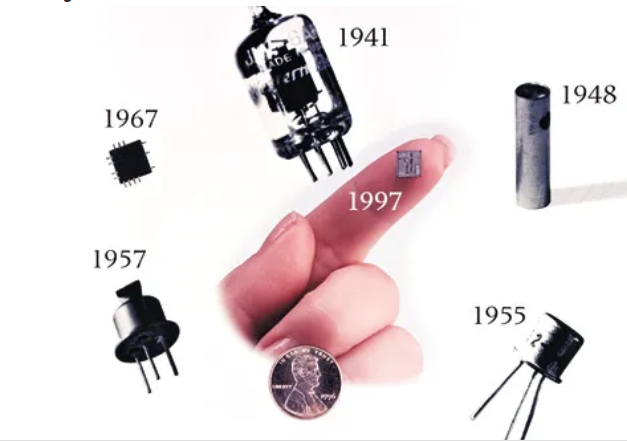
\includegraphics[width=0.5\textwidth]{res/evol_transistor.png}\\
    Evolución del transistor
\end{center}

% \begin{figure}[h]
%     \centering
%     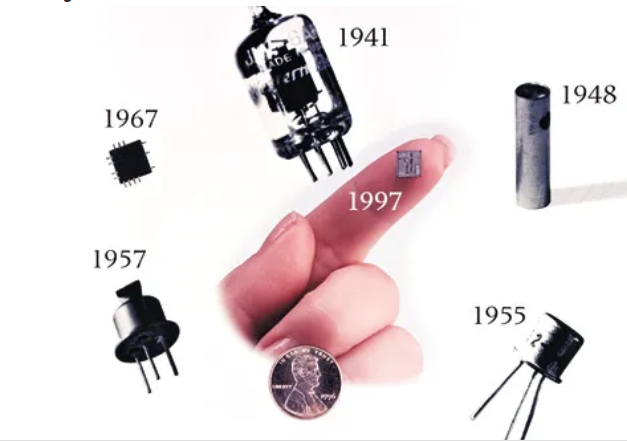
\includegraphics[width=0.5\textwidth]{res/evol_transistor.png}
%     \caption{Evolución del transistor}
%     \label{fig:evol_trans}
% \end{figure}


\section*{Circuito integrado}

Los circuitos integrados (CI), también conocidos como chips, son una pieza clave en la electrónica moderna. 
Los primeros prototipos de CIs se desarrollaron a finales de los años 50 y principios de los 60, 
pero su uso se expandió rápidamente durante la década de 1960. A diferencia de los primeros transistores, 
los circuitos integrados permitieron a los ingenieros combinar varios transistores, diodos y resistencias 
en una sola pieza de silicio.

El primer circuito integrado fue desarrollado por Jack Kilby de Texas Instruments 
y Robert Noyce de Fairchild Semiconductor en 1958. El primer CI contenía sólo un par de transistores, 
pero pronto se desarrollaron chips con docenas, cientos y, finalmente, miles de componentes. 
En 1961, Fairchild Semiconductor lanzó el primer circuito integrado comercial, que contenía 
cuatro transistores y cinco resistencias. En 1964, la empresa japonesa Toshiba comenzó a 
producir circuitos integrados a gran escala, lo que permitió la producción de chips con 
cientos de componentes.

La tecnología de los circuitos integrados sigue evolucionando hoy en día, con chips más pequeños, más rápidos 
y más eficientes energéticamente. La miniaturización y la integración de la electrónica siguen permitiendo 
el desarrollo de tecnologías nuevas e innovadoras.

\begin{center}
    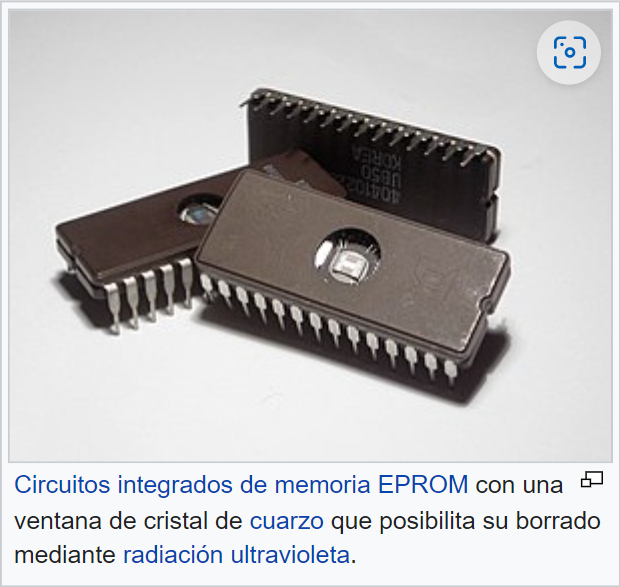
\includegraphics[width=0.5\textwidth]{res/circuito_integrado.png}\\
    Circuito integrado
\end{center}

% \begin{figure}[h]
%     \centering
%     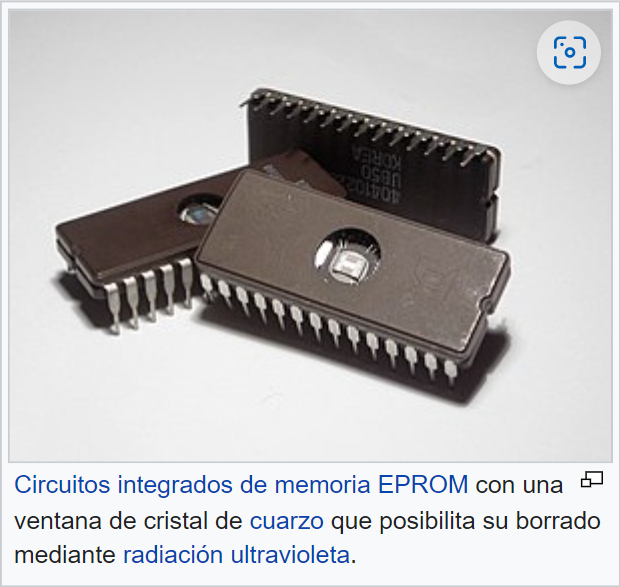
\includegraphics[width=0.5\textwidth]{res/circuito_integrado.png}
%     \caption{Circuito integrado}
%     \label{fig:circ_int}
% \end{figure}

\section*{Microprocesador}
La historia de los microprocesadores comienza a mediados de la década de 1960, cuando se desarrollaron las primeras 
calculadoras electrónicas. Estas calculadoras utilizaban circuitos integrados para realizar operaciones matemáticas, 
pero eran muy costosas y requerían un tamaño considerable para ser operadas. Fue entonces cuando Ted Hoff, 
ingeniero de Intel, propuso la idea de crear un circuito integrado que pudiera realizar múltiples tareas y que fuera accesible 
para el consumidor promedio.

En 1971, Intel presentó el primer microprocesador comercialmente exitoso, el Intel 4004. Este procesador fue diseñado 
para ser utilizado en una calculadora electrónica de mesa japonesa llamada Busicom. Antes de su lanzamiento, 
las calculadoras electrónicas se construían con circuitos integrados específicos para una tarea determinada, 
lo que las hacía costosas y difíciles de producir.

El 4004 era diferente: tenía la capacidad de ejecutar diferentes programas y realizar varias tareas diferentes. 
En términos de especificaciones técnicas, tenía una velocidad de reloj de 740 kHz y un ancho de palabra de 4 bits, 
lo que significa que podía procesar datos de 4 bits a la vez y un total de 2.300 transistores y se fabricó utilizando 
la tecnología de proceso NMOS de 10 micras. El 4004 fue un gran éxito en su época y sentó las bases para la revolución 
de los microprocesadores, para lograrlo, el equipo de Intel utilizó técnicas de diseño innovadoras, como la arquitectura en cascada 
y el uso de multiplexores. Este procesador estableció el estándar para los microprocesadores de 4 bits y allanó el camino 
para el desarrollo  de los microprocesadores de 8 bits y 16 bits en las décadas siguientes. Además, los principios de diseño 
utilizados todavía son relevantes en la fabricación de chips actuales.

En 1972, Intel lanzó el Intel 8008, diseñado por el mismo equipo que creó el 4004. El procesador 8008 tenía un ancho de palabra de 8 bits 
y podía procesar datos a una velocidad de reloj de hasta 800 kHz. Tenía un total de 3.500 transistores y se fabricó utilizando 
la tecnología de proceso NMOS de 10 micras, igual que el 4004. A diferencia del procesador 4004, el 8008 fue diseñado para aplicaciones 
más amplias que incluían sistemas de control industrial y computadoras personales.
Una de las principales mejoras del procesador 8008 fue la capacidad de direccionamiento de memoria mejorada. El 8008 podía direccionar 
hasta 16 KB de memoria RAM, lo que era mucho más que el límite de 16 palabras de 4 bits del procesador 4004.
A pesar de ser un gran avance en su época, el procesador 8008 tenía limitaciones en cuanto a la capacidad de procesamiento, 
lo que hizo que en 1974, Intel lanzara el Intel 8080, que se convirtió en el primer microprocesador de uso general. 
El procesador 8080 tenía una velocidad de reloj de hasta 2 MHz y podía procesar datos a una velocidad de hasta 500.000 
operaciones por segundo. Contaba con un conjunto de instrucciones mejorado en comparación con el procesador 8008, lo que permitía 
una mayor flexibilidad en la programación y el uso de software.

Este procesador también ofreció una mayor capacidad de memoria, pudiendo direccionar hasta 64 KB de memoria RAM. Además, 
tenía una arquitectura de bus de 8 bits, lo que lo hacía compatible con una amplia gama de dispositivos y sistemas.
El 8080 fue utilizado en muchas computadoras personales y sistemas embebidos de la época, incluyendo la popular computadora Altair 8800. 
También se utilizó en aplicaciones militares, sistemas de control industrial y en el sector de la medicina. El éxito del procesador 8080 
sentó las bases para el desarrollo de los procesadores de 16 y 32 bits, y allanó el camino para el auge de la computación personal en la década de 1980. 
De hecho, es considerado por muchos como el "padre" de la familia de procesadores x86, que aún hoy en día es uno de los tipos de procesadores 
más utilizados en las computadoras personales.

Luego en 1978 fue lanzado el Intel 8086, el primer procesador de la familia x86 que marcó un hito en la evolución de los procesadores de computadora. 
Tenía una velocidad de reloj de hasta 10 MHz y podía procesar datos a una velocidad de hasta 1 millón de operaciones por segundo. 
Ofrecía un conjunto de instrucciones más avanzado que su predecesor, el procesador 8080, y permitía una mayor flexibilidad en la programación y 
el uso de software. También ofrecía una capacidad de direccionamiento de memoria de hasta 1 MB, lo que fue un gran avance en comparación con el 8080. 
Además, tenía una arquitectura de bus de 16 bits, lo que lo hacía compatible con una amplia gama de dispositivos y sistemas.
El procesador 8086 fue utilizado en muchos sistemas de la época, incluyendo la popular computadora IBM PC, la primera computadora personal.

A partir de ese momento, los microprocesadores se hicieron cada vez más rápidos y poderosos. En la década de 1980, surgieron los microprocesadores de 32 bits,
 como el Motorola 68000 y el Intel 80386. En la década de 1990, los microprocesadores de 64 bits, como el Intel Pentium Pro y el DEC Alpha, 
 comenzaron a ser utilizados en sistemas informáticos de alto rendimiento. Hoy en día, los microprocesadores son la base de la electrónica moderna, 
 y se utilizan en una amplia variedad de dispositivos, desde telefonos inteligentes y tabletas hasta automóviles y equipos médicos.
\subsection*{Primera generación vs actualidad}
A continuación se ofrece una comparación entre el primer microprocesador comercial de la historia, 
el Intel 4004 y uno de los más avanzados y potentes del mercado actual, el AMD Ryzen 9 5950X. 
El microprocesador Intel 4004 contaba con una capacidad de procesamiento de tan solo 4 bits y una 
velocidad de reloj de 740kHz, además no contaba con unidades de coma flotante ni caché, lo que limitaba 
significativamente su rendimiento. En cambio el AMD Ryzen 9 5950X cuanta con una capacidad de procesamiento
de 64 bits (16 veces superior al Intel 4004) y una velocidad de reloj de hasta 4.9GHz (aproximadamente 6000 veces superior 
al Intel 4004), además de contar con múltiples núcleos y subprocesos, lo que le permite realizar tareas complejas 
y exigentes con una eficiencia impresionante. Los microprocesadores actuales también cuentan con tecnologías avanzadas 
como la inteligencia artificial, la virtualización y la aceleración por hardware, lo que les permite manejar 
grandes cantidades de datos y realizar tareas especializadas con rapidez y precisión. En resumen, la evolución de 
los microprocesadores ha sido impresionante en términos de capacidad de procesamiento, velocidad y tecnologías avanzadas.


\newpage
\section*{Conclusiones}

En conclusión, la historia del transistor, circuito integrado y microprocesador es fascinante e innovadora.  
El transistor permitió la creación de dispositivos electrónicos más pequeños, eficientes y asequibles, 
lo que a su vez condujo al desarrollo de los circuitos integrados y, finalmente, a la invención del microprocesador.
El circuito integrado y el microprocesador son dos de los avances más importantes en la historia de la informática, 
permitiendo la creación de computadoras personales y dispositivos móviles. Además, estos avances han mejorado 
significativamente la eficiencia y la precisión de los sistemas de control y de automatización, lo que ha 
impulsado la industria manufacturera y otros sectores.

A lo largo de la historia, el transistor, el circuito integrado y el microprocesador han sido objeto de una investigación 
y desarrollo continuos, y se espera que sigan evolucionando en el futuro. El impacto de estos avances tecnológicos 
en nuestra sociedad es indudable, y es probable que continúen transformando nuestras vidas 
en formas aún más sorprendentes e inesperadas en los años venideros.
%\begin{thebibliography}{2}

%\bibitem{Wal} \textsc{Walter Isaacson},\textit{Los Innovadores}, Editorial: National Geographic Books, 2019.

%\end{thebibliography}

\bibliography{references}

\end{document}